
%%%%%%%%%%%%%%%%%%%%%%%%%%%%%%%%%%%%%%%%%%%%%%%
% BEGIN GRAVITATIE
%%%%%%%%%%%%%%%%%%%%%%%%%%%%%%%%%%%%%%%%%%%%%%%

\chapter{Gravitatie}

In dit  hoofdstuk wordt het hoogtepunt van de klassieke mechanica behandeld: Newton's
wet van de zwaartekracht. Hoewel het pas ver in de cursus wordt behandeld was het juist
het werk van Newton op het gebied van zwaartekracht, dat de hele klassieke mechanica
echt goed op gang heeft gebracht. Na Newton was de natuurkunde veranderd in een echte
exacte wetenschap.

Stof uit Giancoli:
\begin{itemize}
\item Hoofdstuk 6.1 - 6.5
\item Hoofdstuk 8.7
\end{itemize}

\section{Newton's wet van universele zwaartekracht}

Newton's zwaartekracht wet vertelt je dat twee objecten met $m_1$ en $m_2$ elkaar aantrekken
met een kracht  die evenredig is met beide massa's en omgekeerd evenredig met het kwadraat
van de afstand tussen de objecten. De kracht heeft dezelfde richting als de lijn die de zwaartepunten
van beide objecten verbindt. 

 \begin{figure}[htbp]
\begin{center}
  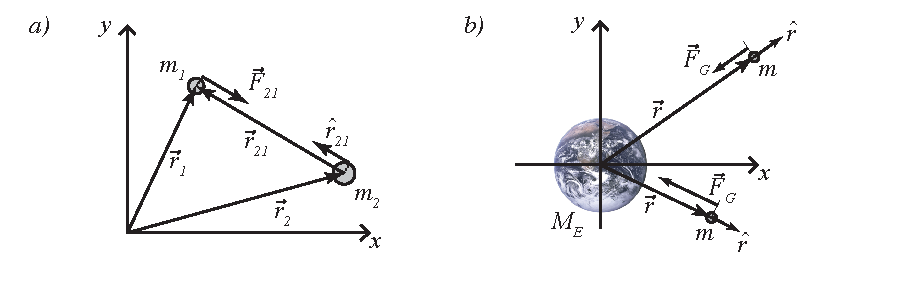
\epsfig{file=NewtonZwaartekracht.pdf, width=\textwidth}
\caption{{\it a) Zwaartekracht uitgeoefend op object~1 door object~2. b) Hetzelfde indien een van de objecten vele malen
zwaarder is dan de andere.}}
\label{fig:NewtonZwaartekracht}
\end{center}
\end{figure} 

In formulevorm ziet Newton's zwaartkrachtwet die wordt uitgeoefend door een willekeurig object met
massa $m_2$ op een ander object met massa $m_1$ er als volgt uit~(zie Fig.~\ref{fig:NewtonZwaartekracht}~a):
\begin{equation}\label{eq:NewtonZwaartekracht}
\vec{F}_{12} = - G\frac{m_1 m_2}{r_{21}^2}\hat{r}_{21}
\end{equation}
De vector $\hat{r}_{21}$ is gedefinieerd als:
\begin{equation}
\hat{r}_{21} \equiv \frac{\vec{r}_{21}}{|\vec{r}_{21}|}= \frac{\vec{r}_1 - \vec{r}_2}{|\vec{r}_1-\vec{r}_2|} 
\end{equation}
Je kan eenvoudig verifieren door de vectoren te tekenen dat $\hat{r}_{21}$ in de richting staat
van object~$1$ gezien vanuit object~$1$: de kracht staat op deze manier in de goede richting omdat
er nog een min-teken staat voor het geheel. Door Newton's wet te gebruiken kan je snel zien dat
 kracht die op object $2$ wordt uitgeoefend door object~$1$ even groot is, maar tegengesteld van 
 teken (\emph{Waarom moet dit wel zo zijn?}). De evenredigheidsconstante $G$ die je ziet voor  
 vgl.~\ref{eq:NewtonZwaartekracht} heet Newton's constante en zijn waarde is:
 \begin{equation}
 G = 6.67\cdot10^{-11}\,N\cdot m^2/kg^2
 \end{equation}
Deze constante zorgt ervoor dat je uiteindelijke kracht de juiste dimensie en grootte in Newtons krijgt. 

In het verder verloop van dit college zullen we meestal 'iets' met zwaartekracht gaan berekenen in het
geval een van de objecten zeer zwaar is, en de andere relatief dus zeer licht. In dat geval kunnen we aannemen
dat het zwaarste van de twee objecten niet significant zal worden beinvloed door het lichtere object. Voor
het gemak, en zonder verlies van precisie kunnen we dan de oorsprong van het coordinatensysteem leggen in het 
centrum van het zware object, en veronderstellen dat dit punt stationair is, zoals getekend in Fig.~\ref{fig:NewtonZwaartekracht}~b).

In het geval van bijvoorbeeld het draaien van een object zoals een satelliet met $m$ om de aarde met $M_E$
is deze benadering uitstekend en reduceert Newtons wet tot:
\begin{equation}\label{eq:NewtonZwaartekracht2}
\vec{F}_{G} = - G\frac{m M_E}{r^2}\hat{r}
\end{equation}
Ook voor bijvoorbeeld de beweging van planeten om de zon is deze benadering prima in de meeste gevallen.
Uiteraard wordt de veronderstelling dat het 'zware' object stilstaat in het centrum van je $CM$ systeem onnauwkeuriger
naarmate de objecten die er omheen draaien zwaarder zijn.

\begin{center}
\line(1,0){250}
\end{center}
\begin{voorbeeld} 
Bepaal met behulp van Newton's wet de massa van de aarde.

{\bf Oplossing: }{\it We weten de valversnelling op het oppervlak van de aarde: $g=9.8m/s^2$. Dus:
\begin{equation}
|\vec{F}_G| = m\,g
\end{equation}
Verder weten we 
de straal van de aarde $r_E=6\cdot 10^6~m$ (Deze kon al tamelijk nauwkeurig worden bepaald door geleerden
in de oudheid. Kan je bedenken hoe ze dat gedaan zouden hebben?). We kunnen vgl.~\ref{eq:NewtonZwaartekracht2} herschrijven tot:
\begin{equation}
M_E = \frac{|\vec{F}_G| r_E^2}{m G}
\end{equation}
Combinatie van de twee vergelijkingen geeft:
\begin{equation}
M_E  =\frac{g \, r_E^2}{G} \approx 5\cdot 10^{24}\,kg
\end{equation}
En dus hebben we de aarde 'gewogen'.
}
\end{voorbeeld}
\begin{center}
\line(1,0){250}
\end{center}

De zwaartekracht zorgt ervoor dat wij naar de aarde worden getrokken, en het is dezelfde kracht die ervoor
zorgt dat planeten om de zon draaien, de maan en satellieten om de aarde, etc etc. We kunnen nu eens kijken 
hoe een object - i.e. satelliet - om de aarde beweegt. Laten we aannemen dat de baan van het object in goede
benadering wordt beschreven met een eenparige cirkelbeweging met straal $r$. We hebben dan volgens 
vgl.~\ref{eq:fc_cirkel} een centripetaalkracht nodig die er uitziet als:
\begin{equation}
\vec{F}_C = -\frac{m\,|\vec{v}|^2}{r}\hat{r}
\end{equation}
Hierin is $|\vec{v}|$ de constante grootte van de baansnelheid.  De enige kracht die de centripetaal versnelling kan
verzorgen is uiteraard de zwaartekracht in dit geval. Dus:
\begin{equation}
-\frac{m\,|\vec{v}|^2}{r}\hat{r} =  - G\frac{m M_E}{r^2}\hat{r}
\end{equation}
Als we de straal van de baan weten kunnen we onmiddellijk de snelheid van de satelliet bepalen:
\begin{equation}
|\vec{v}| = \sqrt{\frac{G M_E}{r}}
\end{equation}
De snelheid hangt niet af van de massa van het object, maar van de massa van de aarde in dit geval, de
zwaartekrachtsconstante, en de straal van de baan. Hoe dichter je bij de aarde komt hoe sneller je 
moet bewegen om in een baan om de aarde te blijven. 

\begin{center}
\line(1,0){250}
\end{center}
\begin{voorbeeld} 
Bereken de straal van de baan van een geostationaire satelliet.

{\bf Oplossing: }{\it We zijn op zoek naar een baan waarvoor geldt dat de omlooptijd net zo lang is als een dag 
op aarde: $T=24~uur$ dus. Als we nu de straal van de baan die we zoeken  $R$ noemen. Dan moet de snelheid gelijk zijn
aan:
\begin{equation}
|\vec{v}| = \frac{2\pi\,R}{T}
\end{equation}
Als we verder aannemen dat de baan cirkelvormig is dan geldt:
\begin{equation}
\frac{|\vec{v}|^2}{R} = \frac{G M_E}{R^2}
\end{equation}
We kunnen nu $|\vec{v}|$ elimineren om te komen tot:
\begin{eqnarray}
\frac{(2\pi\,R)^2}{R\,T^2} & = & \frac{G M_E}{R^2} \\
& \Downarrow & \\
R & = & \left(\frac{G\,M_E\,T^2}{4\pi^2}\right)^{\frac{1}{3}} \approx 4\cdot 10^4~km
\end{eqnarray}

}
\end{voorbeeld}
\begin{center}
\line(1,0){250}
\end{center}

Een belangrijke observatie die je maak als je kijkt naar beelden uit bijvoorbeeld het ISS~\footnote{International
Space Station} is dat alles zich bevindt in een toestand van gewichtsloosheid. Hoe zit dat nou precies? Een
 vaak gehoord argument is dat je gewichtloos bent omdat je ver bent verwijderd van de aarde. Laten we
 eens kijken hoe groot de zwaartekracht ten gevolge van de aarde is als je in het ISS zit. De hoogte waarop
 het ISS rondjes om de aarde draait is ongeveer $h=300~km$ (lage baan dus). Het relatieve verschil van de 
 zwaartekrachtsversnelling op deze hoogte ten opzichte van de versnelling op het aardoppervlak wordt 
 gegeven door:
 \begin{equation}
 \delta \, g \equiv \frac{g(h)-g(h_0)}{g(h_0)} = -\frac{2\,r_E\,h+h^2}{(r_E+h)^2} \approx 5\%
 \end{equation} 
Dat scheelt dus niet zoveel. We moeten ons nu eens afvragen wat gewicht nou precies is. Gewicht is de kracht die
wij uitoefenen op een weegschaal ten gevolge van de zwaartekracht. Als zowel de weegschaal als het object
dat je wil wegen in vrije val zijn, dan drukt het object de weegschaal niet meer in. In vrije val ben je dus
gewichtsloos. Dit is precies hoe een object rond bijvoorbeeld de aarde beweegt: in vrije val. De snelheid van 
het object is in een gesloten baan zodanig dat een object als het ware 'om de aarde' heen valt. Het is dus de hoge
snelheid van een satelliet die ervoor verantwoordelijk is dat deze niet op de aarde stort.

\section{Zwaartekracht potentiele energie}

Laten we nu eens kijken hoe het zit met de arbeid $W$ die je moet verrichten om een object te bewegen
wanneer de zwaartekracht er op werkt. Daarvoor moeten we terugkijken naar de definitie van arbeid zoals
gegeven in vgl.~\ref{eq:defwork}. We zien dat voor de arbeid geldt:
\begin{eqnarray}
W & = & \int_1^2 \vec{F}\cdot d\vec{\ell}\\
    & = &  = - G\,m\,M_E\int_1^2 \frac{\hat{r}\cdot d\vec{\ell}}{r^2}
\end{eqnarray}
 \begin{figure}[htbp]
\begin{center}
  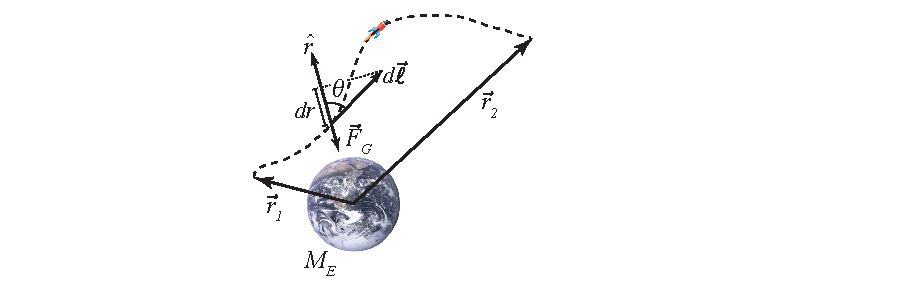
\epsfig{file=NewtonPotentieleEnergie.pdf, width=\textwidth}
\caption{{\it Berekenen van $W$ ten gevolge van zwaartekracht.}}
\label{fig:NewtonPotentieleEnergie}
\end{center}
\end{figure} 
Voor de tweede vergelijking hebben we niets anders gedaan dan het invullen van Newton's zwaartekrachtswet.
De integraal ziet er akelig uit met het inproduct van $\hat{r}$ en $d\vec{\ell}$, dus laten we daar maar eens 
in meer detail naar kijken (zie Fig.~\ref{fig:NewtonPotentieleEnergie}). We kunnen het inproduct schrijven als:
\begin{eqnarray}
\hat{r} \cdot d\vec{\ell} & = & |\hat{r}||d\vec{\ell}|\cos\theta \\ 
& = & |d\vec{\ell}|\cos\theta
\end{eqnarray}
En dit is niets anders dan het stukje van $d\vec{\ell}$ dat in de richting staat van $\hat{r}$, ofwel $dr$. De arbeid
energie schrijven we nu als:
\begin{eqnarray}
W & = & - G\,m\,M_E \int_{|\vec{r}_1|}^{|\vec{r}_2|} \frac{dr}{r^2} \\
     & = & G\,m\,M_E\left(\frac{1}{r_2}-\frac{1}{r_1}\right)
\end{eqnarray}     
De eerste observatie die je hier kan maken is dat de arbeid $W$ alleen maar afhangt van de coordinaten
van het begin en eindpunt van het afgelegde pad. Zwaartekracht is dus een \emph{conservatieve} kracht. Dit
geldt trouwens voor andere soortgelijke centrale krachten, die ook alleen afhangen van $r$, zoals bijvoorbeeld de
elektrische kracht.

Omdat we te maken hebben met een conservatieve kracht, kunnen nu net als in hoofdstuk~\ref{chap:energie} 
een potentiaal identificeren behorend bij de zwaartekracht. Er geldt immers:
\begin{equation}\label{eq:gpot}
\Delta U = -W
\end{equation}
Voor de potentiele zwaartekrachtsenergie kunnen we dus definieren:
\begin{equation}
U(r) = -\frac{G m M_E}{r}
\end{equation}
We zouden een constante waarde kunnen optellen bij onze potentiele energie en nog steeds voldoen
aan vgl.~\ref{eq:gpot}. Deze constante waarde kiezen we 'nul': de moraal is dat alleen verschillen
in potentiele energie relevant zijn, niet de absolute waarde.  We hebben nu onze potentiele energie gedefinieerd
en als een object beweegt onder invloed van de zwaartekracht (geen wrijving en dergelijke) dan
geldt wederom behoud van mechanische energie:
\begin{equation}
K+U=\mbox{Constant}
\end{equation}

\begin{center}
\line(1,0){250}
\end{center}
\begin{voorbeeld} 
Gebruik behoud van energie om de minimale snelheid uit te rekenen zodat een raket afgeschoten vanaf
het aardoppervlak tot $r=\infty$ kan komen.

{\bf Oplossing:}{\it Bij afschieten heeft de raket met snelheid $|\vec{v}_0$ een energie van:
\begin{equation}
E(r=r_E) = K + U = \frac{1}{2}\,m\,|\vec{v}_0|^2-\frac{G\,m\,M_E}{r_E} 
\end{equation}
Met zoals gebruikelijk $M_E$ en $r_E$ de massa en straal van de aarde. Als we willen dat de raket 
naar $r=\infty$ vliegt, dan nemen we maar aan dat $\vec{v}(r=\infty)=\vec{0}$: ofwel de totale energie
is nul als de raket eenmaal oneindig ver weg is gekomen. We moeten dus de snelheid $|\vec{v}_0|$ zodanig
kiezen dat:
\begin{eqnarray}
E(r=r_E) & = & E(r=\infty) = 0 \\
\frac{1}{2}\,m\,|\vec{v}_0|^2-\frac{G\,m\,M_E}{r_E}  & = & 0 \\
& \Downarrow & \\
|\vec{v}_0| & = & \sqrt{\frac{2\,G\,M_E}{r_E}}
\end{eqnarray}
Deze snelheid staat bekend als de ontsnappingssnelheid, en voor de aarde bedraagt deze ongeveer
$11~km/s$ ({\it reken maar na}).
}
\end{voorbeeld}
\begin{center}
\line(1,0){250}
\end{center}

\section{Baanimpulsmoment}

In deze paragraaf wordt iets dieper ingegaan op de beweging van een object ten gevolge van een centrale
kracht (in dit geval zwaartekracht). Deze analyse zal aantonen dat er naast impuls en energie nog een $3^e$
behouden grootheid in het spel is: namelijk het impulsmoment van een object. De afleiding is tamelijk
formeel, dus zet je maar schrap.

We beginnen met het opschrijven van Newtons $2^e$ wet in poolcoordinaten:
\begin{eqnarray}
\vec{F} & = & m\vec{a} \\
\vec{F}_r + \vec{F}_{\phi} & = & m\left(\vec{a}_{r} + \vec{a}_{\phi}\right)
\end{eqnarray}
We hebben nog niets gedaan, behalve het ontbinden van zowel kracht als versnelling in een radiele ($r$)
en een tangentiele ($\phi$) component.  Maar we zien onmiddellijk dat in het geval van een centrale 
kracht, dat $\vec{F}_{\phi}=\vec{0}$: een centrale kracht heeft slechts een radiele component. Nu zie je
waarom het gerbuik van poolcoordinaten in dit geval superieur is boven het gebruik van ordinaire cartesische
coordinaten.  Er valt zomaar een term weg uit je vergelijkingen, terwijl dit in cartesische coordinaten niet
zou gebeuren. Let wel op: je kan natuurlijk het probleem prima beschrijven in cartesische coordinaten en
je zal ook wel dezelfde antwoorden vinden, maar de vergelijkingen die je krijgt  zijn minder 'transparant'. 
Nu kunnen we eens kijken naar de rechterkant van de vergelijking. Met behulp van vgl.~\ref{eq:apool}
krijgen we de volgende twee vergelijkingen:
\begin{equation}
\left\{\begin{array}{ccc}
\vec{F}_r & = & m\left(\frac{d^2r}{dt^2} - r\left(\frac{d\phi}{dt}\right)^2\right)\hat{r} \\
\vec{0} & = & m\left(2 \frac{dr}{dt}\frac{d\phi}{dt}+r\frac{d^2\phi}{dt^2}\right)\hat{\phi}
\end{array}\right.
\end{equation}
Je ziet dat de tweede vergelijking laat zien dat de tangentiele versnelling nul moet zijn. Dit betekent niet dat
de hoek $\phi$ niet verandert. Sterker nog, dit betekent zelfs niet dat $d^2\phi / dt^2=0$(!), zoals je kan zien
aan de vergelijking. Het is nu mogelijk om de vergelijking voor de $\hat{\phi}$ versnelling op vernuftige wijze
te herschrijven als een totale tijdsafgeleide ({\it verifieer deze vergelijking}):
\begin{equation}\label{eq:dLdt}
0 = m\frac{d}{dt}\left(r^2\frac{d\phi}{dt}\right) \hat{\phi} \equiv \frac{dL}{dt} \hat{\phi}
\end{equation}
Het product $m r^2 d\phi/dt$ staat bekend als het baanimpulsmoment van een object, en deze grootheid
hebben we al eerder gezien:
\begin{equation}
L \equiv m r^2 \frac{d\phi}{dt}
\end{equation}
We hebben al eerder gezien dat het impulsmoment een vector is, maar op dit moment is het voldoende om alleen naar de grootte van
deze vector te kijken. Je ziet namelijk in vgl.~\ref{eq:dLdt} dat de afgeleide naar de tijd van het 
impulsmoment nul is. En als de afgeleide nul is moet dus gelden voor een centrale kracht:
\begin{equation}
L = \mbox{constant}
\end{equation}
Als je het impulsmoment op een moment kent, dan ken je deze voor een willekeurig ander moment.
$L$ is namelijk hetzelfde. Voor een eenparige cirkelbeweging is dit evident: de straal van de baan is constant,
net als de hoeksnelheid $d\phi/dt$: $L$ is dus constant. Maar omdat we in onze afleiding geen
enkele aanname hebben gemaakt over de exacte vorm van de baan, geldt behoud van impulsmoment
veel algemener. De meeste planeten in ons zonnestelsel beschrijven geen perfecte cirkelbanen, maar 
ze bewegen over elliptische paden. $L$ is behouden, en je weet dan dat als bijvoorbeeld $r$ voor een
deel van de baan kleiner is, dat op dat moment $d\phi / dt$ dus groter moet zijn. Je kan dit trouwens ook
wel een aanvoelen, omdat een planeet dichter bij de zon minder potentiele energie heeft dan op een
grotere afstand. We weten dat energie is behouden en dus kan het niet anders zijn dan dat de snelheid
voor de kleinere afstand groter is geworden.

\begin{center}
\line(1,0){250}
\end{center}
\begin{voorbeeld} 
Een balletje met massa $m$ is bevestigd aan een touw en draait zonder wrijving rondjes met constante snelheid $\vec{v}_0$
op afstand $r_0$ zoals in Fig.~\ref{fig:ImpulsMoment}. Door aan het touw te trekken wordt de afstand $r_1$. Wat is nu de
snelheid $|\vec{v}_1|$?
 \begin{figure}[htbp]
\begin{center}
  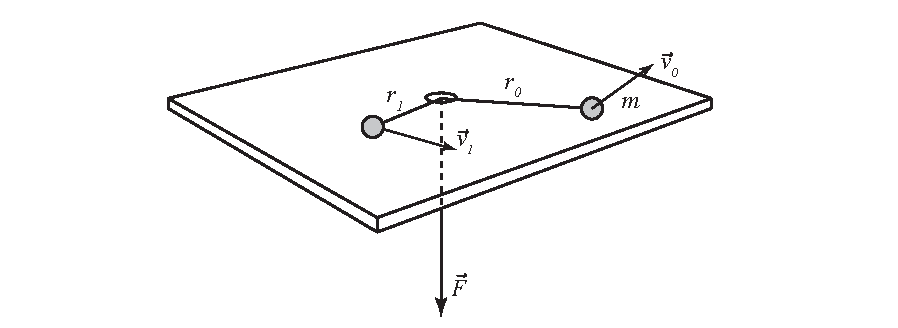
\epsfig{file=ImpulsMoment.pdf, width=\textwidth}
\caption{{\it Behoud van impulsmoment voor een balletje aan een touw.}}
\label{fig:ImpulsMoment}
\end{center}
\end{figure} 

{\bf Oplossing: }{\it  Het balletje wordt in de bocht gehouden door de centripetaalkracht die wordt geleverd door aan het 
touw te trekken met kracht $\vec{F}$. De centripetaalkracht is alleen radieel gericht en dus is impulsmoment behouden.
Op $t=0$ geldt:
\begin{equation}
L = m r_0^2 \frac{d\phi}{dt} = m r_0^2 \frac{|\vec{v}_0|}{r_0} = m r_0 |\vec{v}_0|
\end{equation}
Waarbij we gebruiken dat $\vec{v}_ = (d\phi / dt) r_0 \hat{\phi}$. Nadat de straal is veranderd naar $r_1$ geldt:
\begin{equation}
L = m r_1 |\vec{v}_1|
\end{equation}
En dus:
\begin{equation}
|\vec{v}_1| = |\vec{v}_0| \frac{r_0}{r_1}
\end{equation}
}
\end{voorbeeld}
\begin{center}
\line(1,0){250}
\end{center}

\section{Banen van de planeten}

Dit hoofdstuk wordt afgesloten met een korte beschouwing van de beweging van objecten bij een centrale kracht,
zoals bijvoorbeeld geldt voor de beweging van een planeet m de zon. We kijken hiervoor naar de totale energie
van een object $E$, die zoals wij weten behouden is int dit geval. Dus:
\begin{equation}\label{eq:etot_grav}
E = \frac{1}{2}m|\vec{v}|^2 + U(r)
\end{equation}
De kinetische energie $K$ wordt geschreven als (\emph{volg afleiding maar eens stap voor stap}) :
\begin{eqnarray}
\frac{1}{2} m|\vec{v}|^2 & = & \frac{1}{2}m (\vec{v}_{r}+\vec{v}_{\phi})\cdot(\vec{v}_{r}+\vec{v}_{\phi}) \\
& = & \frac{1}{2}m (\vec{v}_r\cdot\vec{v}_r + 2 \vec{v}_r\cdot\vec{v}_{\phi} + \vec{v}_{\phi}\cdot\vec{v}_{\phi}) \\ 
& = & \frac{1}{2}m (|\vec{v}_r|^2 + |\vec{v}_{\phi}|^2) \\
& = & \frac{1}{2}m\left\{\left(\frac{dr}{dt}\right)^2+r^2\left(\frac{d\phi}{dt}\right)^2\right\} \\
& = & \frac{1}{2}m\left\{\left(\frac{dr}{dt}\right)^2+\frac{L^2}{(m\,r)^2}\right\}
\end{eqnarray}
We hebben dus de kinetische energie herschreven in een term met de radiele snelheid en het impulsmoment. Dit
gaat ons enorm helpen in verdere berekeningen omdat $L$ niet verandert. Als we deze uitdrukking voor de
kinetische energie invullen in vgl.~\ref{eq:etot_grav} krijgen we:
\begin{equation}
E = \frac{1}{2} m\left(\frac{dr}{dt}\right)^2+\frac{L^2}{2\,m\,r^2} + U(r) \equiv \frac{1}{2} m\left(\frac{dr}{dt}\right)^2 + U_{eff}(r)
\end{equation}
Hoewel je dat misschien niet meteen ziet, kan deze uitdrukking worden gebruikt om op te lossen langs wat voor 
pad een object in een centrale potentiaal beweegt. We kunnen namelijk een uitdrukking vinden voor $dr/dt$:
\begin{equation}
\frac{dr}{dt} = \sqrt{\frac{2}{m}\left(E-U_{eff}(r)\right)}
\end{equation}
Verder kunnen we de definitie van $L$ gebruiken om ook voor $d\phi / dt$ een mooie uitdrukking te vinden:
\begin{eqnarray}
L & = & m r^2 \left(\frac{d\phi}{dt}\right)^2 \\
& \Downarrow & \\
\frac{d\phi}{dt} & = & \frac{L}{m\,r^2}
\end{eqnarray}
Door combinatie van de twee laatste vergelijkingen krijgen we een uitdrukking die de baan van bijvoorbeeld
een planeet  beschrijft:
\begin{equation}
\frac{d r}{d\phi} = \frac{\sqrt{(2/m)(E-U_{eff}(r))}}{L/mr^2}
\end{equation}
Deze vergelijking hangt alleen maar af van $r$, terwijl de waarden van de totale energie en het impulsmoment
voor een bepaalde baan van een object moeten worden vastgelegd, of gekozen (ze veranderen niet). Het blijkt
dat de krommen die $r$ beschrijven als functie van $\phi$ ofwel cirkelbanen, ofwel ellipsen ofwel hyperbolen 
zijn~\footnote{Afleiding hiervan bevat geen nieuwe fysische concepten, maar is geometrisch lastig. Slaan we voor dit
college over.} 
De baan van de maan om de aarde, en van de planeten om de zon, maar ook het vallen van objecten op
aarde kunnen op deze manier door Newton's wet van universele zwaartekracht worden beschreven. Deze beschrijving
van meerdere fysische observaties vanuit een universeel principe is een fenomenale doorbraak in de natuurkunde 
geweest.

\section{Wat moet ik weten en kunnen?}

Na dit hoofdstuk moet je weten:
\begin{itemize}
\item Hoe een centrale kracht eruit ziet, en in het bijzonder de Newton's zwaartekrachtswet.
\item Hoe de potentiele energie eruit ziet voor een centrale kracht. 
\item Wat impulsmoment is.
\item Waarom Newton een 'grote jongen' is.
\end{itemize}
Je moet kunnen:
\begin{itemize}
\item Rekenen met centrale krachten en bijbehorende potentiele energie.
\item Rekenen met impulsmoment.
\end{itemize}

\section{Opgaven}

\begin{enumerate}
\item Doorlezen Giancoli paragraaf 6-5.
\item Giancoli Hoofdstuk 6: 11, 16, 17, 18, 34, 63, 66, 69, 70, 74, 
\item Giancoli Hoofdstuk 8: 45, 47, 48, 52, 58, 60, 99, 100,  
\item Bepaal het gewicht van iemand met massa $m$ die (i) op de noordpool van de aarde staat en die (ii) op
de evenaar van de aarde staat.
\end{enumerate}

%%%%%%%%%%%%%%%%%%%%%%%%%%%%%%%%%%%%%%%%%%%%%%%
% EINDE GRAVITATIE
%%%%%%%%%%%%%%%%%%%%%%%%%%%%%%%%%%%%%%%%%%%%%%%
